\documentclass[10pt,a4paper]{beamer}

% theme %

\usetheme[compress]{Dresden}
\usefonttheme{professionalfonts}

% color definitions %

\definecolor{Board}{RGB}{60,145,143}
\definecolor{DoubleWordBonus}{RGB}{239,174,154}
\definecolor{DoubleLetterBonus}{RGB}{141,201,240}
\definecolor{TripleLetterBonus}{RGB}{54,156,219}
\definecolor{Tile}{RGB}{247,225,190}
\definecolor{UniGreen}{RGB}{0,150,0}

% slide colors setup %

\setbeamercolor{title}{fg=UniGreen}
\setbeamercolor{frametitle}{fg=UniGreen}
\setbeamercolor{structure}{fg=UniGreen}

% import statements %

\usepackage[utf8]{inputenc}
\usepackage[MeX]{polski}
\usepackage{amsmath}
\usepackage{amsfonts}
\usepackage{amssymb}
\usepackage{graphicx}
\usepackage{rotating}
\usepackage{multirow}
\usepackage{array}
\usepackage{adjustbox}
\usepackage{caption}
\usepackage{ragged2e}
\usepackage{tikz}
\usetikzlibrary{calc,shapes,shapes.multipart,arrows,chains}

% cool timeline %

\definecolor{arrowcolor}{RGB}{0,150,0}
\definecolor{circlecolor}{RGB}{255,255,255}
\colorlet{textcolor}{black}
\definecolor{bordercolor}{RGB}{220,0,0}

\pgfdeclarelayer{background}
\pgfsetlayers{background,main}

\newcounter{task}

\newlength\taskwidth% width of the box for the task description
\newlength\taskvsep% vertical distance between the task description and arrow

\setlength\taskwidth{2.5cm}
\setlength\taskvsep{17pt}

\def\taskpos{}
\def\taskanchor{}

\newcommand\task[1]{%
  {\parbox[t]{\taskwidth}{\scriptsize\Centering#1}}}

\tikzset{
inner/.style={
  on chain,
  circle,
  inner sep=4pt,
  fill=circlecolor,
  line width=1.5pt,
  draw=bordercolor,
  text width=1.2em,
  align=center,
  text height=1.25ex,
  text depth=0ex
},
on grid
}

\newcommand\Task[2][]{%
\node[inner xsep=0pt] (c1) {\phantom{A}};
\stepcounter{task}
\ifodd\thetask\relax
  \renewcommand\taskpos{\taskvsep}\renewcommand\taskanchor{south}
\else
  \renewcommand\taskpos{-\taskvsep}\renewcommand\taskanchor{north}
\fi
\node[inner,font=\footnotesize\sffamily\color{textcolor}]    
  (c\the\numexpr\value{task}+1\relax) {#1};
\node[anchor=\taskanchor,yshift=\taskpos] 
  at (c\the\numexpr\value{task}+1\relax) {\task{#2}};
}

\newcommand\drawarrow{% the arrow is placed in the background layer 
                                                     % after the node for the tasks have been placed
\ifnum\thetask=0\relax
  \node[on chain] (c1) {}; % if no \Task command is used, the arrow will be drawn
\fi
\node[on chain] (f) {};
\begin{pgfonlayer}{background}
\node[
  inner sep=10pt,
  single arrow,
  single arrow head extend=0.8cm,
  draw=none,
  fill=arrowcolor,
  fit= (c1) (f)
] (arrow) {};
\fill[white] % the decoration at the tail of the arrow
  (arrow.before tail) -- (c1|-arrow.west) -- (arrow.after tail) -- cycle;
\end{pgfonlayer}
}

\newenvironment{timeline}[1][node distance=.75\taskwidth]
  {\par\noindent\begin{tikzpicture}[start chain,#1]}
  {\drawarrow\end{tikzpicture}\par}

% page numbers %

\expandafter\def\expandafter\insertshorttitle\expandafter{%
  \insertshorttitle\hfill\insertframenumber\,/\,\inserttotalframenumber}

\usepackage{tikz-uml}

\author[Jakub Turek]{\texorpdfstring{Jakub Turek \newline \href{mailto:J.Turek@stud.elka.pw.edu.pl}{ J.Turek@stud.elka.pw.edu.pl }}{Jakub Turek} \newline \vskip2pt {\small Promotor: dr inż. Jakub Koperwas}}
\title{Zaawansowana sztuczna inteligencja do gry Scrabble}
\institute{Wydział Elektroniki i~Technik Informacyjnych}
\date{25 kwietnia 2014}
\begin{document}

\begin{frame}
	\titlepage
\end{frame}

\section{Wprowadzenie}
\subsection{Agenda}

\begin{frame}
	\frametitle{Agenda}

	\begin{enumerate}
		\item Wprowadzenie.
			\begin{enumerate}
				\item Ogólny opis Scrabble.
				\item Spis zagadnień omówionych na pierwszym seminarium.
			\end{enumerate}
		\item Omówienie podstaw teoretycznych.
			\begin{enumerate}
				\item Optymalna strategia.
				\item Podział na fazy gry.
			\end{enumerate}
		\item Opis wykorzystywanych algorytmów w~podziale na fazy gry.
		\item Wyniki testów.
		\item Podsumowanie.
			\begin{enumerate}
				\item Literatura uzupełniająca.
 			\end{enumerate}
	\end{enumerate}
\end{frame}

\subsection{O~Scrabble}

\begin{frame}
	\frametitle{Scrabble - definicja}

	\begin{itemize}
		\item Gra planszowa dla 2-4 osób.
		\item Na początku gry każdy gracz otrzymuje po 7~klocków. Klocki należą do jednej z~dwóch grup:
			\begin{itemize}
				\item Reprezentują pojedynczą literę alfabetu i~przypisaną do niej wartość punktową.
				\item Reprezentują dowolną literę i~nie mają wartości punktowej (blanki).
			\end{itemize}
		\item Gra toczy się w~turach. W~każdej turze zadaniem gracza jest ułożenie na planszy wyrazu w~układzie krzyżówkowym:
			\begin{itemize}
				\item Dopuszczalne są dowolne wyrazy lub ich odmiany ujęte w~słownikach języka i~ortograficznych.
				\item Wyjątki stanowią wyrazy rozpoczynające się wielką literą, skróty, przedrostki, przyrostki oraz słowa wymagające użycia łącznika lub apostrofu. 
			\end{itemize}
		\item Wartość punktowa jest zależna od sumy wartości klocków oraz ich położenia na planszy (premie literowe oraz słowne).
	\end{itemize}
\end{frame}

\begin{frame}
	\frametitle{Plansza do gry}

	\begin{figure}
		\centering
		\includegraphics[scale=0.17]{graphics/board.jpg}
		\caption{Plansza wykonana z~włókna węglowego, podświetlana diodami LED.}
	\end{figure}
\end{frame}

\subsection{Turnieje}

\begin{frame}
	\frametitle{Scrabble jako gra turniejowa w~Polsce}

	\begin{itemize}
		\item Polska Federacja Scrabble to oficjalna federacja zrzeszająca kluby Scrabble w~Polsce. Została założona w~1997 roku.
		\item Ranking PFS zrzesza 335 graczy, którzy rozegrali minimum 30 partii turniejowych w~przeciągu ostatnich dwóch lat.
		\item Zasady:
			\begin{itemize}
				\item Ograniczony czas na wykonanie wszystkich ruchów - po 20 minut na gracza.
				\item Dozwolone są ruchy uznawane za poprawne przez Oficjalny Słownik Polskiego Scrabblisty.
			\end{itemize}
		\item Rekordy:
			\begin{itemize}
				\item Najwyższy wynik w~partii pełnej - Michał Alabrudziński, 721 punktów.
				\item Najlepsze otwarcie - Radosław Sowiński, 112 punktów za słowo \textbf{źrebień}.
			\end{itemize}
	\end{itemize}
	
\end{frame}

\subsection{Ekstrakt z~SDM1}

\begin{frame}
	\frametitle{Przypomnienie (1/2)}

	Podczas poprzedniego wystąpienia zostały omówione następujące zagadnienia:

	\begin{enumerate}
		\item Porównanie słowników do gier dla języka polskiego:
			\begin{description}
				\item[OSPS] ,,Oficjalny Słownik Polskiego Scrabblisty''.
				\item[SA] Słownik alternatywny.
			\end{description}
		\item Analiza statystyczna słownika alternatywnego.
		\item Omówienie efektywnych struktur słownikowych zorientowanych na przeglądanie poprawnych sufiksów wyrazów:
			\begin{description}
				\item[Trie] Drzewo poszukiwań.
				\item[DAG] Directed Acyclic Graph.
				\item[GADDAG] prefiksowo-sufiksowa odmiana DAG.
			\end{description}
	\end{enumerate}
\end{frame}

\begin{frame}
	\frametitle{Przypomnienie (2/2)}

	Omówione zagadnienia - ciąg dalszy:

	\begin{enumerate}
		\setcounter{enumi}{3}
		\item Przedstawienie algorytmu Appela-Jacobsona wyznaczającego wszystkie legalne kombinacje ruchów dla ustalonego stanu gry.
		\item Porównanie najlepszych algorytmów sztucznej inteligencji obecnej generacji:
			\begin{itemize}
				\item Algorytm Maven.
				\item Aplikacja Quackle.
			\end{itemize}
		\item Przedstawienie wybranych elementów algorytmu używanego w~aplikacji Quackle.
	\end{enumerate}
\end{frame}

\subsection{Założenia}

\begin{frame}
	\frametitle{Założenia algorytmu}
	
	Cel pracy oraz przyjęte założenia:

	\begin{itemize}
		\item Zwiększenie procentowej liczby wygranych najlepszych algorytmów obecnej generacji:
			\begin{itemize}
				\item Skuteczność mierzona w~starciu z~przeciwnikami klasy mistrzowskiej.
			\end{itemize}
		\item Algorytmem bazowym (oraz referencyjnym) jest wykorzystywany przez aplikację Quackle.
		\item Średni czas wykonania ruchu nie może być większy niż w~algorytmach obecnej generacji.
		\item Złożoność pamięciowa algorytmu nie jest istotna.
		\item Słownik dopuszczalnych wyrazów jest znany z~góry:
			\begin{itemize}
				\item Dodanie obsługi nowego języka wymaga przeprowadzenia automatycznej analizy, która może być operacją czasochłonną.
			\end{itemize}
	\end{itemize}
\end{frame}

\section{Podstawy teoretyczne}
\subsection{Strategia optymalna}

\begin{frame}
	\frametitle{Strategia optymalna}

	\begin{block}{Twierdzenie}	
		Istnieje optymalna strategia gry w~Scrabble.
	\end{block}

	\begin{block}{Przestrzeń stanów}	
		Stan rozgrywki po~danej turze opisują parametry $P$ - rozmieszczenie klocków na planszy oraz $Z$ - zagranie. Przejście między stanami determinuje zmiana $(\Delta P, \Delta Z)$.
	\end{block}

	\begin{block}{Dowód}	
		Dla dowolnej rozgrywki tworzymy graf możliwych stanów wychodząc 
		od stanu końcowego. Do stanu końcowego można wejść tylko poprzez skończoną liczbę legalnych zagrań. Rozumując iteracyjnie dochodzimy do stanu początkowego, na każdym etapie analizując skończoną liczbę przejść między stanami. Wynika z~tego, że ilość stanów jest skończona. Można więc w~każdym kroku wybrać optymalną strategię, która maksymalizuje prawdopodobieństwo wygranej.
	\end{block}
\end{frame}

\begin{frame}
	\frametitle{Strategia optymalna - ilustracja dowodu}
	
	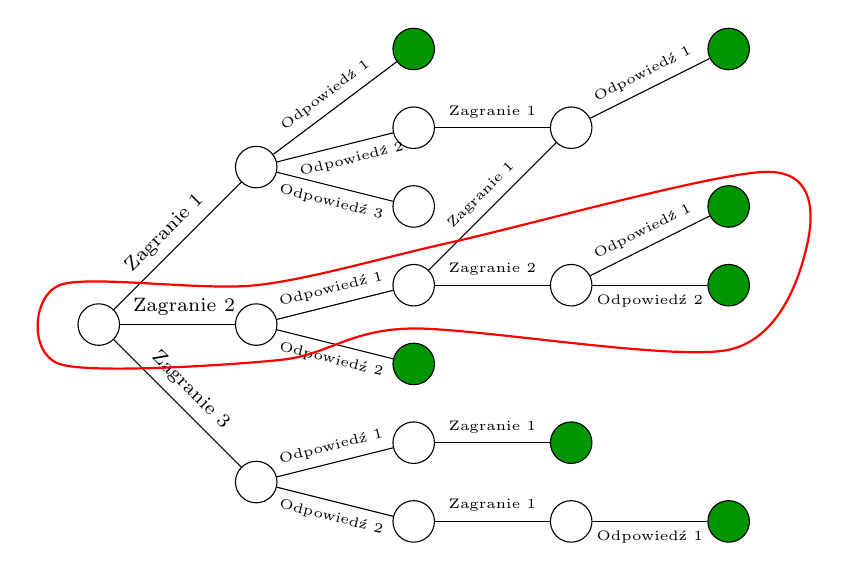
\begin{tikzpicture}
		\tikzstyle{state} = [draw, shape=circle, minimum width=15pt, minimum height=15pt]
		\node (s0) [state] at (0,0) {};
		\node (s1) [state] at (2,2) {};
		\node (s2) [state] at (2,0) {};
		\node (s3) [state] at (2, -2) {};
		\node (s4) [state, fill=UniGreen] at (4,3.5) {};
		\node (s5) [state] at (4,2.5) {};
		\node (s6) [state] at (4,1.5) {};
		\node (s7) [state] at (4,0.5) {};
		\node (s8) [state, fill=UniGreen] at (4,-0.5) {};
		\node (s9) [state] at (4,-1.5) {};
		\node (s10) [state] at (4,-2.5) {};
		\node (s11) [state] at (6,2.5) {};
		\node (s12) [state] at (6,0.5) {};
		\node (s13) [state, fill=UniGreen] at (6,-1.5) {};
		\node (s14) [state] at (6,-2.5) {};
		\node (s15) [state, fill=UniGreen] at (8,3.5) {};
		\node (s16) [state, fill=UniGreen] at (8,1.5) {};
		\node (s17) [state, fill=UniGreen] at (8,0.5) {};
		\node (s18) [state, fill=UniGreen] at (8,-2.5) {};
		\draw (s0) -- node[above, sloped, font=\scriptsize] {Zagranie 1} (s1);
		\draw (s0) -- node[above, sloped, font=\scriptsize, near end, xshift=-8pt] {Zagranie 2} (s2);
		\draw (s0) -- node[above, sloped, font=\scriptsize] {Zagranie 3} (s3);
		\draw (s1) -- node[above, sloped, font=\tiny] {Odpowiedź 1} (s4);
		\draw (s1) -- node[xshift=-6pt, below, near end, sloped, font=\tiny] {Odpowiedź 2} (s5);
		\draw (s1) -- node[below, sloped, font=\tiny] {Odpowiedź 3} (s6);
		\draw (s2) -- node[above, sloped, font=\tiny] {Odpowiedź 1} (s7);
		\draw (s2) -- node[below, sloped, font=\tiny] {Odpowiedź 2} (s8);
		\draw (s3) -- node[above, sloped, font=\tiny] {Odpowiedź 1} (s9);
		\draw (s3) -- node[below, sloped, font=\tiny] {Odpowiedź 2} (s10);
		\draw (s5) -- node[above, sloped, font=\tiny] {Zagranie 1} (s11);
		\draw (s7) -- node[above, sloped, font=\tiny] {Zagranie 1} (s11);
		\draw (s7) -- node[above, sloped, font=\tiny] {Zagranie 2} (s12);
		\draw (s9) -- node[above, sloped, font=\tiny] {Zagranie 1} (s13);
		\draw (s10) -- node[above, sloped, font=\tiny] {Zagranie 1} (s14);
		\draw (s11) -- node[above, sloped, font=\tiny] {Odpowiedź 1} (s15);
		\draw (s12) -- node[above, sloped, font=\tiny] {Odpowiedź 1} (s16);
		\draw (s12) -- node[below, sloped, font=\tiny] {Odpowiedź 2} (s17);
		\draw (s14) -- node[below, sloped, font=\tiny] {Odpowiedź 1} (s18);
		\draw [red, thick] plot [smooth cycle] coordinates {(-0.5, -0.5) (-0.5, 0.5) (2, 0.5) (4.5, 1.05) (8.5, 1.94) (9, 1.03) (8, -0.32) (3.96, -0.05) (2.3, -0.45)};
	\end{tikzpicture}
\end{frame}

\begin{frame}
	\frametitle{Strategia optymalna - następstwa}

	\begin{itemize}
		\item Wyznaczenie optymalnej strategii należy do klasy problemów \emph{PSPACE-complete}.
		\item Analiza przestrzeni stanów jest możliwa wyłącznie dla bardzo ograniczonej przestrzeni stanów:
			\begin{itemize}
				\item W~praktyce analiza przestrzeni stanów jest możliwa, gdy w~worku nie ma już klocków lub gdy pozostał jeden/dwa klocki.
			\end{itemize}
		\item \textbf{Należy zmieniać strategię w~zależności od fazy rozgrywki}:
			\begin{itemize}
				\item Nie zawsze można użyć strategii optymalnej.
				\item Wykorzystanie metod heurystycznych.
			\end{itemize}
	\end{itemize}
\end{frame}

\subsection{Fazy gry}

\begin{frame}
	\frametitle{Fazy gry}
	
	Rozgrywkę w~Scrabble można podzielić na cztery zasadnicze fazy:

	\begin{description}
		\item[OP] \emph{opening-play}. Faza obejmuje pierwsze zagranie.
		\item[MG] \emph{mid-game}. Faza trwa od momentu rozpoczęcia rozgrywki do momentu rozpoczęcia fazy \emph{pre-endgame}.
		\item[PEG] \emph{pre-endgame}. Faza rozpoczyna się, gdy w~worku pozostaje $\leq 7$ klocków i~trwa do rozpoczęcia fazy \emph{end-game}. W~PEG każde kolejne zagranie może poskutkować opróżnieniem worka. Dodatkowy podział:
			\begin{description}
				\item[PEG-1] W~worku pozostał jeden klocek. Przez tę fazę przechodzi około $50\%$ gier.
				\item[PEG-2] W~worku pozostały dwa klocki.
				\item[PEG-X] W~worku pozostało $x \leq 7$ klocków.
			\end{description}
		\item[EG] \emph{end-game}. W~worku nie ma już żadnych klocków.
	\end{description}
\end{frame}

\captionsetup[figure]{skip=10pt}

\begin{frame}[fragile]
	\frametitle{Strategia a~faza gry}
	
	\begin{figure}
		\centering
		\begin{timeline}
			\Task[OP]{Maksymalizacja punktów uzyskanych z~zagrania otwierającego}
			\Task[MG]{Algorytm z~heurystyczną funkcją kosztu i~symulacją w~przód}
			\Task[PEG]{Złączenie algorytmów dla MG i~EG}
			\Task[EG]{Przeszukiwanie przestrzeni stanów (z~ograniczeniami)}
		\end{timeline}
		\caption{Zmiana strategii wraz z~progresją rozgrywki.}
	\end{figure}
\end{frame}

\subsection{Strategia}

\begin{frame}[fragile]
	\frametitle{Wzorzec projektowy - strategia}
	
	\begin{columns}
		\begin{column}{.5\textwidth}
			\begin{block}{Strategia}	
				Wzorzec definiuje rodzinę algorytmów, pakuje je jako osobne klasy i~powoduje, że są one w~pełni wymienne. Zastosowanie strategii pozwala na to, aby zmiany w~implementacji przetwarzania były całkowicie niezależne od strony klienta, który z~nich korzysta.
			\end{block}
		\end{column}
		\begin{column}{.5\textwidth}
			\scalebox{0.7}{
				\begin{tikzpicture}
					\tikzumlset{fill class=white!100}
					\umlclass[type=interface,x=0,y=3]{ScrabbleAI}{\# phase : GamePhase}{+ move() : void \\ \# pickStrategy() : IMoveStrategy} 
					\umlclass[type=interface,x=0,y=0]{IMoveStrategy}{}{+ move() : void} 
					\umlclass[x=-2, y=-2.25]{FirstPlayStrategy}{}{+ move() : void}
					\umlclass[x=0, y=-4.5]{MidGameStrategy}{}{+ move() : void}
					\umlclass[x=2, y=-2.25]{EndGameStrategy}{}{+ move() : void}
					\umluniassoc{ScrabbleAI}{IMoveStrategy}
					\umlimpl{IMoveStrategy}{FirstPlayStrategy}
					\umlimpl{IMoveStrategy}{MidGameStrategy}
					\umlimpl{IMoveStrategy}{EndGameStrategy}
				\end{tikzpicture}
			}
		\end{column}
	\end{columns}
\end{frame}

\section{Algorytmy}
\subsection{Faza opening-play}

\begin{frame}
	\frametitle{Otwarcie gry}

	\begin{itemize}
		\item Celem jest wybranie najwyżej punktowanego zagrania.
		\item W~algorytmie aplikacji Quackle jest przeszukiwany słownik i~dla każdej prawidłowej kombinacji liter wyznaczana jest wartość punktowa.
		\item Wprowadzona optymalizacja wydajnościowa:
			\begin{itemize}
				\item Ponieważ słownik jest znany z~góry można przeprowadzać wstępne obliczenia.
				\item Każdą możliwą kombinację liter indeksujemy 7-wyrazowym ciągiem znaków, które przedstawiają litery ułożone w~porządku alfabetycznym.
				\item Dla każdego indeksu obliczamy najlepsze otwarcie.
				\item Najlepsze otwarcie wyznaczane w~czasie jednostkowym (wyjątek: blanki).
			\end{itemize}
	\end{itemize}
\end{frame}

\subsection{Faza mid-game}
\captionsetup[figure]{skip=2pt}

\begin{frame}
	\frametitle{Algorytm dla fazy mid-game}

	\begin{figure}
		\centering
			\scalebox{0.57}{
				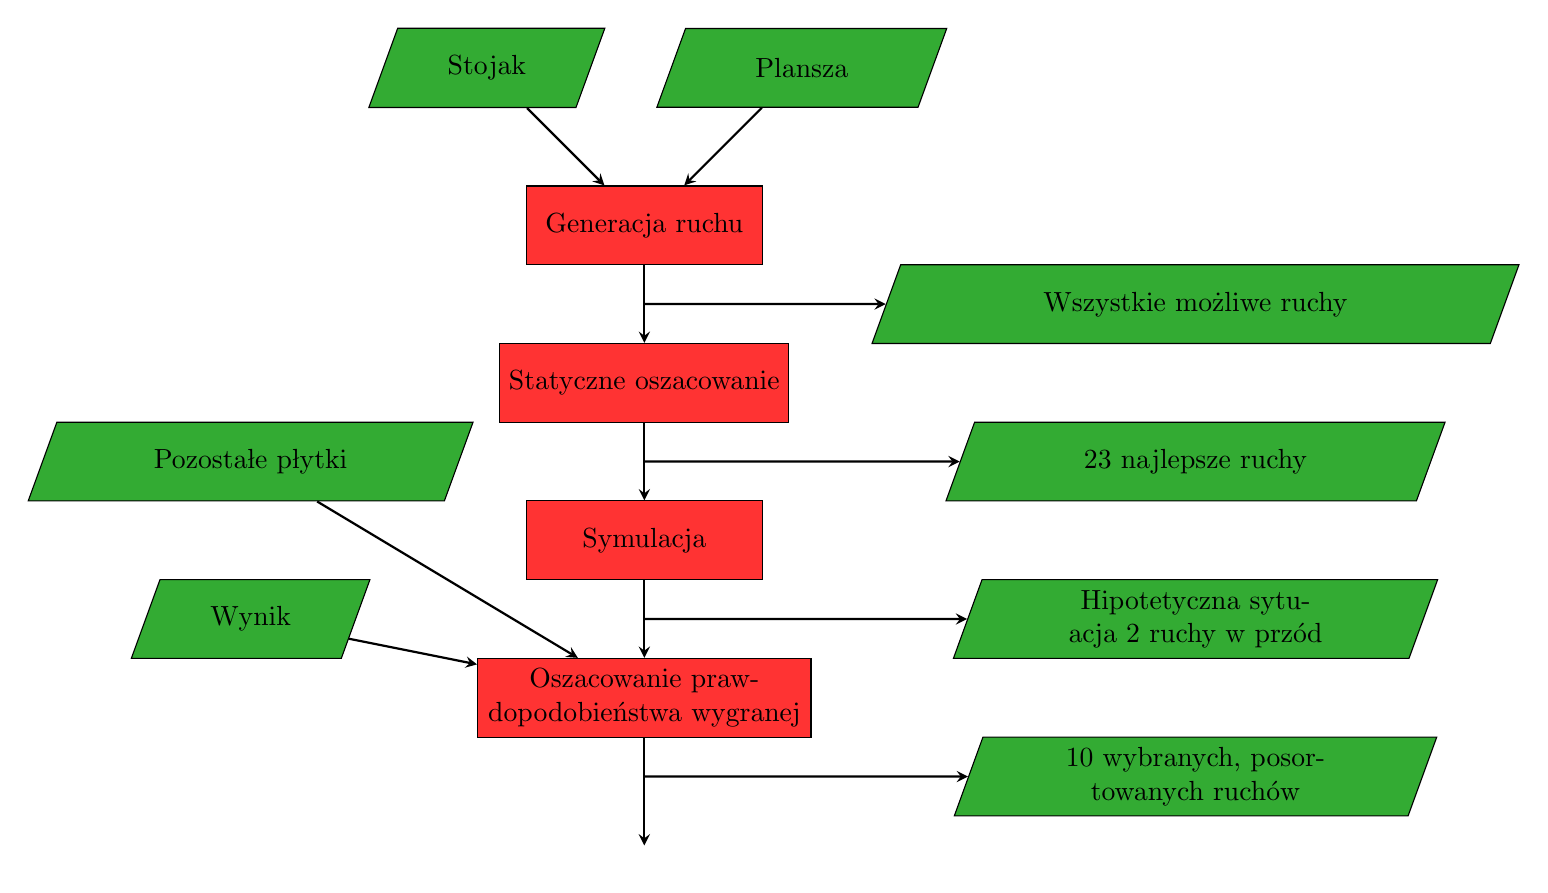
\begin{tikzpicture}[node distance=2cm]
					\noindent
					\tikzstyle{io} = [trapezium, trapezium left angle=70, trapezium right angle=110, minimum width=3cm, minimum height=1cm, text centered, draw=black, fill=UniGreen!80]
					\tikzstyle{process} = [rectangle, minimum width=3cm, minimum height=1cm, text centered, draw=black, fill=red!80]
					\tikzstyle{arrow} = [thick,->,>=stealth]
					
					\node (rack) [io] {Stojak};
					\node (board) [io, right of=rack, xshift=2cm] {Plansza};
					\coordinate (rackboard) at ($(rack)!0.5!(board)$);
					\node (movegen) [process, below of= rackboard] {Generacja ruchu};
					\node (staticeval) [process, below of=movegen] {Statyczne oszacowanie};
					\coordinate (movegenstaticeval) at ($(movegen)!0.5!(staticeval)$);
					\node (possmoves) [io, right of=movegenstaticeval, xshift=5cm] {Wszystkie możliwe ruchy};
					\node (simulation) [process, below of=staticeval] {Symulacja};
					\node (bestmoves) [io, below of=possmoves] {23 najlepsze ruchy};
					\node (hypsequences) [io, below of=bestmoves, text width=5cm] {Hipotetyczna sytuacja 2 ruchy w~przód};
					\node (winpercestimation) [process, below of=simulation, text width=4cm] {Oszacowanie prawdopodobieństwa wygranej};
					\node (end) [process, draw=none, fill=none, below of=winpercestimation, minimum height=1mm] { };
					\coordinate (staticevalsimulation) at ($(staticeval)!0.5!(simulation)$);
					\node (tilesleft) [io, left of=staticevalsimulation,xshift=-3cm] {Pozostałe płytki};
					\node (score) [io, below of=tilesleft] {Wynik};
					\coordinate (winpercestimationend) at ($(winpercestimation)!0.5!(end)$);
					\node (chosenmoves) [io, below of=hypsequences,text width=5cm] {10 wybranych, posortowanych ruchów};
					\draw [arrow] (movegen) -- (staticeval);
					\draw [arrow] (staticeval) -- (simulation);
					\draw [arrow] (simulation) -- (winpercestimation);
					\draw [arrow] (rack) -- (movegen);
					\draw [arrow] (board) -- (movegen);
					\draw [arrow] (winpercestimation) -- (end);
					\draw [arrow] (tilesleft) -- (winpercestimation);
					\draw [arrow] (score) -- (winpercestimation);
					\draw [arrow] ($(movegen)!0.5!(staticeval)$) -- (possmoves);
					\draw [arrow] ($(staticeval)!0.5!(simulation)$) -- (bestmoves);
					\draw [arrow] ($(simulation)!0.5!(winpercestimation)$) -- (hypsequences);
					\draw [arrow] ($(winpercestimation)!0.5!(end)$) -- (chosenmoves);
				\end{tikzpicture}
			}
			\caption{Schemat algorytmu referencyjnego dla fazy MG.}
	\end{figure}
\end{frame}

\begin{frame}
	\frametitle{Faza mid-game: statyczne oszacowanie}
	
	Algorytm referencyjny wykorzystuje do statycznego oszacowania poniższą funkcję celu.

	\begin{block}{Funkcja celu}	
		$F(x) = P(x) + LV(x)$,
		\vskip5pt
		gdzie $P(x)$ to liczba punktów za zagranie $x$, a~$LV(x)$ to \emph{leave value} klocków pozostałych po wykonaniu zagrania $x$. 
	\end{block}

	\begin{block}{Leave value}	
		Obliczona na podstawie bazy danych gier wartość, która faworyzuje kombinacje liter o~większym prawdopodobieństwie dopełnienia wysokopunktowych zagrań w~nadchodzących ruchach. Może przyjmować dodatnie oraz ujemne wartości.
	\end{block}
\end{frame}

\begin{frame}
	\frametitle{Faza mid-game: symulacja}

	Algorytm referencyjny wykonuje następującą symulację:

	\begin{enumerate}
		\item Gracz wykonuje zagranie $P_{1}$.
		\item Przeciwnik wybiera 7~losowych klocków, wyznacza wszystkie możliwości ruchu i~wykonuje zagranie $P_{2}$ dla ruchu z~najlepszym statycznym oszacowaniem.
		\item Gracz uzupełnia klocki, wyznacza wszystkie możliwości ruchu i~wykonuje zagranie $P_{3}$ dla ruchu z~najlepszym statycznym oszacowaniem.
		\item Gracz oblicza wartość $PV_{1}$ zagrania $P_{1}$ odejmując od liczby swoich punktów po zagraniu $P_{3}$ liczbę punktów przeciwnika po zagraniu $P_{2}$.
		\item Gracz dodaje do $PV_{1}$ \emph{leave value} po zagraniu $P_{3}$.
	\end{enumerate}
\end{frame}

\begin{frame}
	\frametitle{Faza mid-game: oszacowanie prawdopodobieństwa wygranej}
	
	Algorytm referencyjny szacuje prawdopodobieństwo wygranej zgodnie z~poniższą zależnością.

	\begin{block}{Estymata prawdopodobieństwa wygranej}	
		$W: PV, TR \rightarrow [0;1]$,
		\vskip5pt
		gdzie $PV$ to wartość zagrania obliczona na etapie symulacji, a~$TR$ to liczba klocków pozostałych do wykorzystania w~partii.
	\end{block}

	Wartość funkcji jest wyznaczana na podstawie bazy danych gier.
\end{frame}

\begin{frame}
	\frametitle{Faza mid-game: słabe strony algorytmu (1/2)}

	Symulacja pomija istotne aspekty rozgrywki:

	\begin{itemize}
		\item Zawartość stojaka jest losowana z~pozostałej puli klocków z~użyciem rozkładu jednostajnego. Można lepiej wyznaczyć rozkład prawdopodobieństwa:
		\begin{itemize}
			\item W~poprzednim ruchu przeciwnik ułożył słowo \textbf{RADO}. Łatwo wywnioskować, że nie posiadał on liter \textbf{U} oraz \textbf{I}, gdyż w~przeciwnym razie prawdopodobnie ułożyłby lepiej punktowane słowa - \textbf{URODA} lub \textbf{RADIO}.
			\item Trzy litery są pozostałością po poprzednim ruchu, więc przy ich losowaniu wykluczamy z~worka \textbf{U} oraz \textbf{I}.
		\end{itemize}
		\item Symulacja nie uwzględnia zjawiska \emph{łowienia} korzystnych zagrań:
		\begin{itemize}
			\item Niektóre kombinacje liter dają $90\%$ prawdopodobieństwo, że po dobraniu do nich kolejnych liter będzie można ułożyć cenny 7-literowy wyraz.
			\item Próba przewidzenia klocków przeciwnika przy podejrzeniu \emph{łowienia}.
		\end{itemize}
	\end{itemize}
\end{frame}

\begin{frame}
	\frametitle{Faza mid-game: słabe strony algorytmu (2/2)}
	
	Oszacowanie prawdopodobieństwa wygranej wykorzystuje nieprecyzyjne informacje wejściowe:

	\begin{itemize}
		\item Pozycja ,,w~przyszłości'' wyznaczona na etapie symulacji może być nieadekwatna do rzeczywistości:
		\begin{itemize}
			\item W~trakcie symulacji pominięte zostało \emph{bingo} przeciwnika.
		\end{itemize}
		\item Podział zagrań na ofensywne i~defensywne na podstawie ilości otwartych premii oraz ilości otaczających klocków po wykonaniu zagrania.
		\item Rozważanie opłacalności zagrania ofensywnego / defensywnego na obecnym etapie rozgrywki. 
		\begin{itemize}
			\item Wykorzystanie sieci neuronowej.
		\end{itemize}
	\end{itemize}
	
\end{frame}

\subsection{Faza end-game}

\begin{frame}
	\frametitle{Faza end-game (1/2)}
	
	\begin{itemize}
		\item Możliwe wykorzystanie drzewa przestrzeni stanów:
		\begin{itemize}
			\item Dla rozgrywki 7~na 7~klocków ilość gałęzi wynosi 200, a~maksymalna ilość zagłębień wynosi 14.
			\item Nie można zastosować efektywnie algorytmu $\alpha - \beta$.
			\item Wymagane jest przeszukiwanie drzewa z~ograniczeniami.
		\end{itemize}
		\item Wykorzystanie programowania dynamicznego:
			\begin{itemize}
				\item Założenie, że sytuacja na planszy jest statyczna. Szacowana jest wyłącznie wartość stojaków.
				\item Wartość każdego możliwego ruchu jest szacowana przy założeniu, że gra zakończy się dokładnie w~$N$ turach.
				\item Oszacowanie wartości ruchu $F_{N}(x) = P_{N}(x) + LV_{N-1}$, gdzie $P_{N}$ to liczba punktów uzyskanych za ruch, a~$LV_{N-1}$ to oszacowanie wartości pozostałych klocków przy założeniu, że do końca gry pozostało $N-1$ tur.
			\end{itemize}
	\end{itemize}
\end{frame}

\begin{frame}
	\frametitle{Faza end-game (2/2)}
	
	Przykład oszacowania:

	\begin{enumerate}
		\item Gracz 1~($G_{1}$) zakończy grę w~8 ruchach. Wtedy gracz 2~($G_{2}$) rozegra 7~ruchów. Powstaje ścieżka, którą przetwarzamy algorytmem minimax.
		\item $G_{2}$ zakończy grę w~7~ruchach. $G_{1}$ rozegra wtedy 7~ruchów. Jeżeli ta ścieżka będzie lepsza dla $G_{2}$, $G_{2}$ wybierze właśnie ją.
		\item $G_{1}$ będzie miał okazję do poprawy jeżeli zakończy grę w~7~ruchach...
	 \end{enumerate}

	 Algorytm jest powtarzany do momentu, gdy żaden z~graczy nie może się poprawić.
\end{frame}

\begin{frame}
	\frametitle{Faza end-game: modyfikacje}
	
	\begin{itemize}
		\item Nie zawsze istnieje jedna optymalna ścieżka zagrania dla przeciwnika:
		\begin{itemize}
			\item Przykładowo, jeżeli przeciwnik może zagrać słowo \textbf{ALE} w~dwóch pozycjach (za 25 i~28 punktów) korzyść z~zablokowania drugiej pozycji względem zablokowania pierwszej  wynosi tylko 3~punkty.
		\end{itemize}
		\item Rozwiązaniem problemu jest wprowadzenie dwóch oszacowań:
		\begin{itemize}
			\item optymistycznego,
			\item pesymistycznego.
		\end{itemize}
		\item Wykorzystanie algorytmu $B^{*}$ do przeszukiwania przestrzeni (minimax nie wspiera przedziałów).
	\end{itemize}
\end{frame}

\subsection{Faza pre-endgame}

\begin{frame}
	\frametitle{Faza pre-endgame}
	
	Algorytm w~fazie \emph{pre-endgame} wymaga połączenia podejść wykorzystywanych w~fazach \emph{mid-game} i~\emph{end-game}:

	\begin{itemize}
		\item Obliczenia wykonywane w~fazie \emph{mid-game} nadal pozostają poprawne.
		\item Istnieje możliwość zakończenia gry w~dwóch turach, więc dla uzyskania pełnego obrazu należy przeszukać przestrzeń stanów jak w~fazie \emph{end-game}.
		\item Hybrydowy algorytm dla fazy \emph{pre-endgame} jest uruchamiany począwszy od 9~klocków pozostałych w~worku.
	\end{itemize}
\end{frame}

\section{Testowanie}
\subsection{Wyniki testów}

\begin{frame}
	\frametitle{Wyniki testów przeciwko algorytmowi referencyjnemu}

	\begin{columns}
		\begin{column}{.45\textwidth}
			\begin{itemize}
				\item 1523 rozegrane partie.
				\item Teoretyczny rozkład dla przeciwników na jednakowym poziomie powinien być bliski $50\%-50\%$.
				\item Wyraźne odchylenie na korzyść algorytmu po modyfikacjach.
			\end{itemize}
		\end{column}
		\begin{column}{.55\textwidth}
			\scalebox{0.8}{
				\begin{tabular}{|l|c|c|}
					\hline
									& 	Algorytm		&	Algorytm		\\
									& 	zmodyfikowany 	& 	referencyjny 	\\
					\hline
					Wygrane 		& 	987				& 	536				\\
					\hline
					\% wygranych	&   \textbf{64,8\%} & 	35,2\%			\\
					\hline
				\end{tabular}
			}
		\end{column}
	\end{columns}
\end{frame}

\begin{frame}
	\frametitle{Wyniki testów przeciwko ludziom}
	
	\begin{itemize}
		\item Nie udało się przeprowadzić miarodajnych testów przeciwko ludziom.
		\begin{itemize}
			\item Przewaga, którą daje znajomość całego słownika jest tak duża, że algorytm osiągnął $100\%$ wygranych w~dotychczasowych rozgrywkach przeciwko ludziom.
			\item Niemożność przeprowadzenia testów na przeciwnikach klasy mistrzowskiej.
		\end{itemize}
		\item W~przyszłości skuteczność algorytmu testowana będzie przeciwko graczom serwisu \href{http://www.kurnik.pl}{kurnik.pl}.
	\end{itemize}
	
\end{frame}

\section{Podsumowanie}
\subsection{Literatura uzupełniająca}

\begin{frame}
	\frametitle<presentation>{Literatura uzupełniająca}
	\begin{thebibliography}{10}
		\beamertemplatearticlebibitems
			\bibitem{ScrabblePSPACE}
    		M.~Lampis, V.~Mitsou, K.~Sołtys.
    		\newblock Scrabble is PSPACE-Complete.

		\beamertemplatebookbibitems
			\bibitem{WCCS}
			Brian Sheppard.
			\newblock World-championship-caliber Scrabble.
			\newblock {\em Artificial Intelligence}, vol. 134, p. 241-275, January 2002.
  		
  		\beamertemplatearticlebibitems
  			\bibitem{Quackle2005}
  			J.~Katz-Brown, J.~O'Laughlin.
    		\newblock How Quackle Plays Scrabble.
	\end{thebibliography}
\end{frame}

\subsection{Zakończenie}

\begin{frame}
	\begin{center}
		\LARGE{\textbf{Dziękuję za uwagę!}}
	\end{center}
\end{frame}

\end{document}